% Charlotte Geiger - Manuel Lippert - Leonard Schatt
% Physikalisches Praktikum

% Teilauswertung 1

\section{Reflexion an Glas}
Bei der ersten Teilaufgabe bestimmen wir den Brechungsindex von Glas, indem wir den Brewsterwinkel gemessen haben. 
Die Beziehung zwischen den Brechindices und dem Brewsterwinkel ist folgendermaßen:\\
\begin{equation}
\theta_B=tan^{-1}\biggl( \frac{n_2}{n_1}\biggr)=tan^{-1}(n_2)  \tab \text{mit} n_1=1
\end{equation}
Aus dem Protokollbuch kann man folgenden Wert für den Brewsterwinkel entnehmen:\\
Die Fehler sind:\\
Für den Winkel $\varphi$: 
Ablesefehler $s_a=\pm1^\circ$\\
Bei der Spannung U: Ablesefehler: $s_a=\pm0,5 Digits$, Systematischer Fehler: $s_r=0,02\% + 4Digits$\\
Schwankung ist bei parallele Polarisation $\pm0,02mV$, bei senkrechter: $\pm0,1mV$\\

Da die Schwankung im Gegensatz zum Ablesefehler sowohl bei der parallelen, als auch bei der senkrechten Polarisation durchschnittlich mindestens um einen Faktor 150 kleiner ist, vernachlässigen wir diese Unsicherheit.\
Mit dem Fehlerfortpflanzungsgesetz folgt:\
\begin{equation}
s_\varphi=\sqrt{s_a^2}=1^\circ
\end{equation}
\begin{equation}
s_U=\sqrt{s_a^2+s_r^2}=\sqrt{(0,5*U)^2+(0,0002*U+0,0004)^2}
\end{equation}
Nach der Theorie, die wir auch schon in den Fragen zur Vorbereitung beschrieben haben, muss die  Spannung der gemessenen Intensität beim Brewsterwinkel bei paralleler Polarisation gegen Null gehen. Bei unserer Messung haben wir dieses Phänomen bei dem\\
\begin{equation}
\theta = 54^\circ
\end{equation}
\begin{equation}
\boxed{U_{p}=(34\pm17)10^{-1} mV}
\end{equation}
erreicht. Wir haben zwar nicht genau die Spannung Null erreicht, aber mit dem Fehler des Winkels und der Spannung, sowie die Schwankung der Spannung fällt dieser Wert deutlich noch in die Messungenauigkeit und liegt in der Fehlertoleranz. \\
Daher folgt:\\
\begin{equation}
\theta_B=54^\circ=tan^{-1}(n_2) \tab \Leftrightarrow \tab n_2=tan(\theta_B)=1,37638
\end{equation}
\begin{equation}
s_{n_2}=s_{\theta_B}=0,017455
\end{equation}
\begin{equation}
\boxed{n_2=(137\pm2)10^{-3}}
\end{equation}
Im Vergleich zu handelsüblichem Glas wie zum Beispiel Kalk-Natron-Silikatglas ca. 1,5, für Borosilikatglas ca. 1,47 und für Aluminosilikatglas ca. 1,5 sieht man, das unserer berechnete Wert in der Fehlertoleranz von dem Brechindex von Glas liegt. Diese Messmethode ist daher ausreichend genau für eine Brechindexbestimmung. \\
\footnote{\url{https://www.baunetzwissen.de/glossar/b/brechungsindex-51605}}

Mit Hilfe des bestimmten Brechindex des Glases und der Fresnelschen Formeln bestimmen wir nun die theoretische Abhängigkeit von den folgenden Formeln, wobei $E_{r,\parallel}$ bzw. $E_{r,\perp}$ die reflektierte und $E_{e,\parallel}$ bzw. $E_{e,\perp}$ die einfallende Energie bezeichnen. 
\begin{equation}
\frac{E_{r,\parallel}}{E_{e,\parallel}}  
\end{equation}
\begin{equation}
\frac{E_{r,\perp}}{E_{e,\perp}}
\end{equation}
Mit der Beziehung $\frac{U}{U_e}=\frac{I}{I_e}$ und den dazugehörigen Fehlern berechnen wir nun zuerst die Werte mit den folgenden Formeln aus dem Skript:
\begin{equation}
\biggl( \frac{E_{r,\parallel}}{E_{e,\parallel}} \biggr)=\sqrt{\frac{I_{r,\parallel}}{I_{e,\parallel}}} = \sqrt{\frac{U}{U_e}}
\end{equation}
\begin{equation}
\biggl( \frac{E_{r,\perp}}{E_{e,\perp}} \biggr)=\sqrt{\frac{I_{r,\perp}}{I_{e,\perp}}}=\sqrt{\frac{U}{U_e}}
\end{equation}
Mit dem Fehlerfortpflanzungsgesetz:
\begin{equation}
s_{\frac{E_r}{E_e}}=\frac{1}{2}\sqrt{\frac{s^2_{I_r}}{I_eI_r}+\frac{I_rs_{I_e}}{I_e^2}}
\end{equation}
Somit bekommen wir die Werte in der folgenden Tabelle:
\begin{center}
    \captionof{table}{Messreihe für parallele Polarisation}
    \begin{tabular}{l | c c c c}
        {} & $\varphi/\circ$ & $U_{p,theo}/~\text{mV}$ & $U_{p}/~\text{mV}$ & $s_{U_{p}}/~\text{mV}$\\
        \hline
        1  & 15 & 0.1502 & 0.1906 & 0.0511 \\
        2  & 20 & 0.1435 & 0.0228 & 0.0322 \\
        3  & 25 & 0.1344 & 0.1428 & 0.0420 \\
        4  & 30 & 0.1225 & 0.1421 & 0.0419 \\
        5  & 35 & 0.1072 & 0.1415 & 0.0418 \\
        6  & 40 & 0.0877 & 0.1207 & 0.0389 \\
        7  & 45 & 0.0629 & 0.0905 & 0.0357 \\
        8  & 50 & 0.0314 & 0.0577 & 0.0334 \\
        9  & 53 & 0.0084 & 0.0218 & 0.0322 \\
        10 & 54 & 0.0000 & 0.0070 & 0.0320 \\
        11 & 55 & 0.0088 & 0.0095 & 0.0320 \\
        12 & 56 & 0.0182 & 0.0100 & 0.0320 \\
        13 & 57 & 0.0280 & 0.0115 & 0.0320 \\
        14 & 60 & 0.0607 & 0.0390 & 0.0326 \\
        15 & 65 & 0.1280 & 0.1207 & 0.0389 \\
        16 & 70 & 0.2163 & 0.2088 & 0.0554 \\
        17 & 75 & 0.3332 & 0.3503 & 0.1060 \\
        18 & 80 & 0.4901 & 0.4795 & 0.1774 \\
        19 & 85 & 0.7038 & 0.6985 & 0.3511 \\
    \end{tabular}
    \captionof{table}{Messreihe für senkrechte Polarisation}
    \begin{tabular}{l | c c c c}
        {} & $\varphi/\circ$ & $U_{s,theo}/~\text{mV}$ & $U_{s}/~\text{mV}$ & $s_{U_{s}}/~\text{mV}$\\
        \hline
        1  & 15 & 0.16 & 0.22 & 0.05 \\
        2  & 20 & 0.17 & 0.23 & 0.06 \\
        3  & 25 & 0.18 & 0.24 & 0.06 \\
        4  & 30 & 0.19 & 0.26 & 0.06 \\
        5  & 35 & 0.20 & 0.28 & 0.07 \\
        6  & 40 & 0.22 & 0.29 & 0.08 \\
        7  & 45 & 0.25 & 0.32 & 0.09 \\
        8  & 50 & 0.28 & 0.36 & 0.11 \\
        9  & 55 & 0.31 & 0.40 & 0.12 \\
        10 & 60 & 0.36 & 0.44 & 0.14 \\
        11 & 65 & 0.42 & 0.51 & 0.19 \\
        12 & 70 & 0.49 & 0.58 & 0.23 \\
        13 & 75 & 0.58 & 0.67 & 0.31 \\
        14 & 80 & 0.69 & 1.03 & 0.70 \\
        15 & 85 & 0.83 & 0.87 & 0.51 \\
    \end{tabular}
    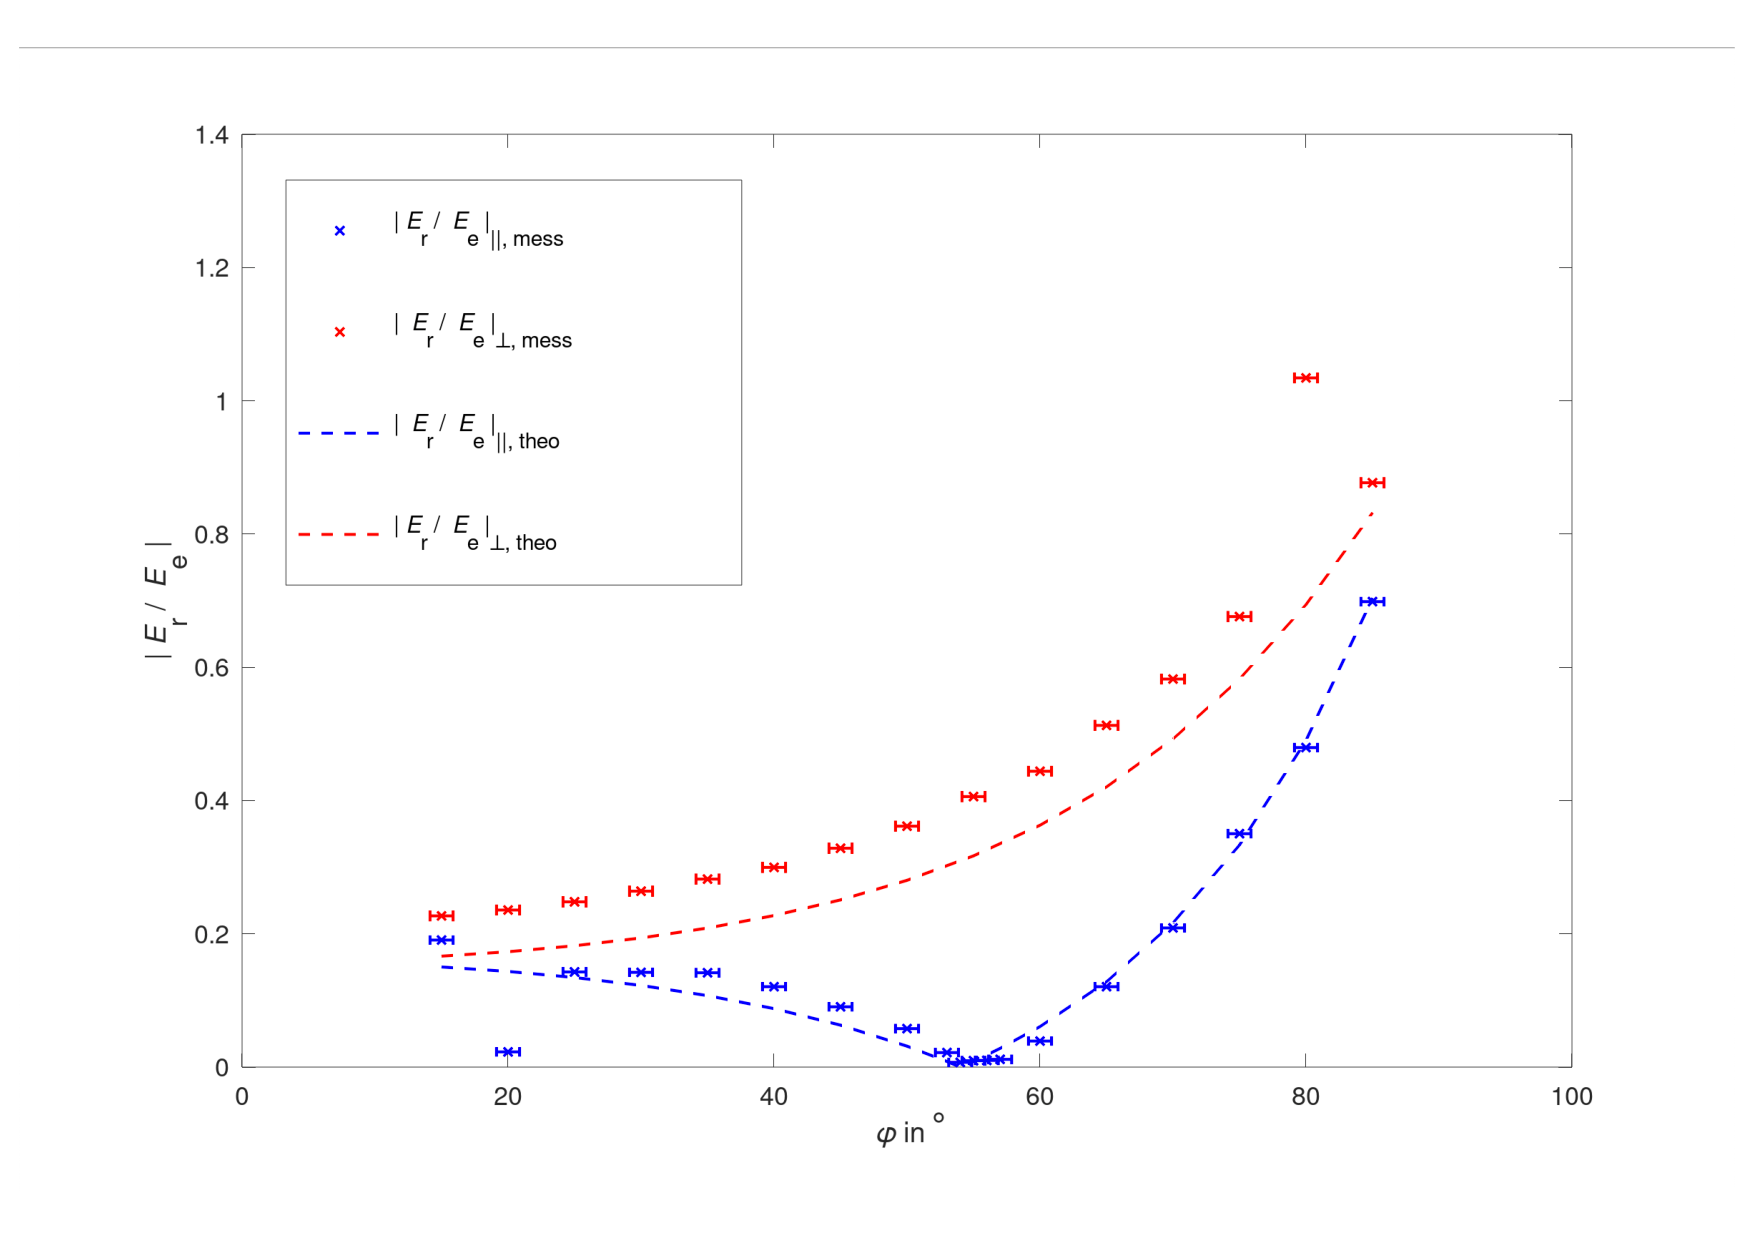
\includegraphics[scale=0.5]{IntPlot.pdf}
    \captionof{figure}{Test} %TODO
\end{center}
Man erkennt in der Graphik, dass unserer Kurvenverlauf dem theoretischen Verlauf sehr ähnelt, jedoch erkennt man auch vor allem bei der Roten Linie, daher bei der senkrechten Polarisation einen deutlichen Abstand zur theoretischen Linie. Da dieser Abstand durchgehend nahezukonstant bleibt, vermuten wir einen von systematischen Fehler dahinter.  Die Gründe für die Abweichungen sind vor allem die Lichtverschmutzung in dem Raum, denn trotz guter Abschirmung des Experimentaufbaus war es unmöglich ihn komplett abzuschirmen. Ausschlaggebend dafür ist das beispielsweise das Aufblicken der Messperson um die Werte zu erfragen und dem damit verbundenen Lichtstrahl der Stirnlampe. Zusätzlich ging die Tür zu dem Raum des Öfteren auf, wodurch zusätzliches Licht in den Raum drang.  Auch sind die Messungenauigkeiten des Messapparat relativ hoch, was sich durch das Fehlerfortpflanzungsgesetz durch alle Werte zieht. 
Es gibt bei unseren Messungen zwei Werte, die deutlich aus der Statistik herausfallen. Zum Einen ist das der Wert der parallelen Polarisation bei $20 \circ$, der wahrscheinlich durch ein verrutschtes Komma zustande gekommen ist. Zusätzlich erkennt man einen falsch liegenden Wert bei $80\circ$ bei der senkrechten Polarisation. Dieser Wert ist unmöglich, da sich das Verhältnis von $E_r$ zu $E_e$ über eins befindet, wodurch man raus schließt, dass die Reflektierte Intensität größer sein müsste als die einfallende Intensität, was physikalisch nicht möglich ist. Der falsche Wert dieses Messwertes ist wohl auch auf eine Misskommunikation zwischen Messperson und Protokollperson zurückzuführen.